\section{色彩迁移实验}

\subsection{色彩迁移方法}
\begin{frame}{当前章节}
    \tableofcontents[currentsection, currentsubsection]
\end{frame}

\begin{frame}{色彩迁移方法} 
    \begin{description}
        \item[HM] histogram matching 经典直方图匹配方法
        \item[reinhard] color transfer between images, 2001, 在正交的$I, \alpha, \beta$空间中变换
        \item[MKL] Monge-Kantorovich Linearization, 2007, 最优传输的思想引入色彩迁移
        \item[MVGD] Multi-Variate Gaussian Distributions, 在色彩迁移中引入多元高斯分布, 2007
    \end{description}
    
\end{frame}

\subsection{色彩迁移实验结果}

\begin{frame}{当前章节}
    \tableofcontents[currentsection, currentsubsection]
\end{frame}

\begin{frame}{色彩迁移实验结果}
    \begin{figure}[!htbp]
        \centering
        \subfloat[hm]{\label{fig:0101a}
        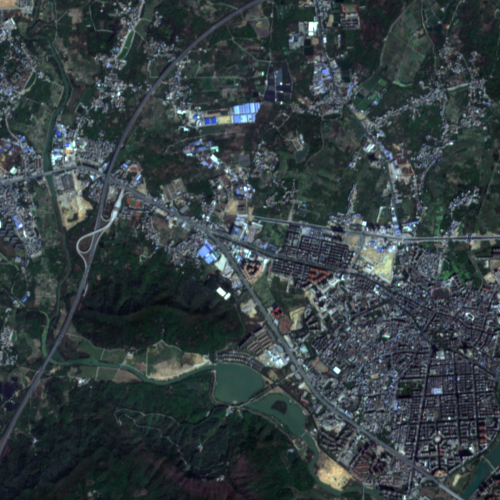
\includegraphics[height=2.5cm]{pic/pic01_hm.png}}
        \quad
        \subfloat[reinhard]{\label{fig:0101b}
        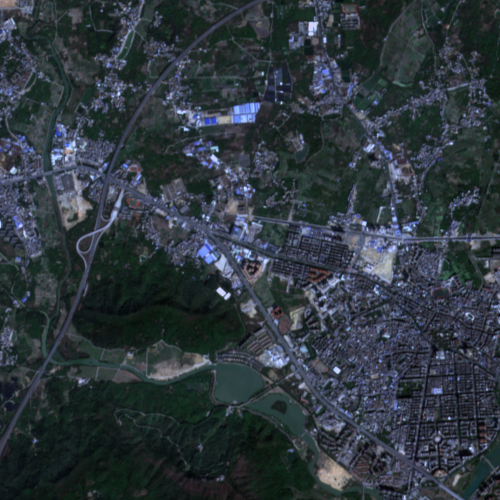
\includegraphics[height=2.5cm]{pic/pic01_reinhard.png}}
        \\[0.1cm]
        \subfloat[mkl]{\label{fig:0101a}
        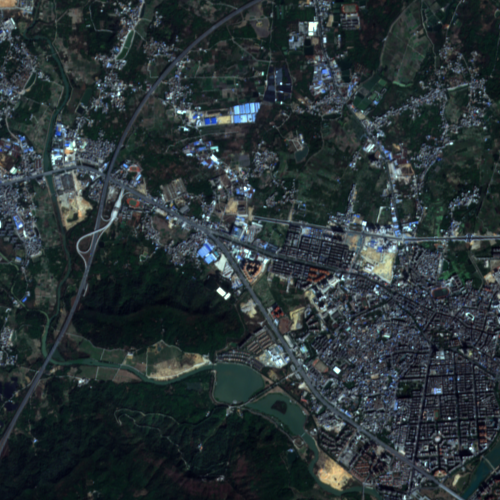
\includegraphics[height=2.5cm]{pic/pic01_mkl.png}}
        \quad
        \subfloat[mvgd]{\label{fig:0101b}
        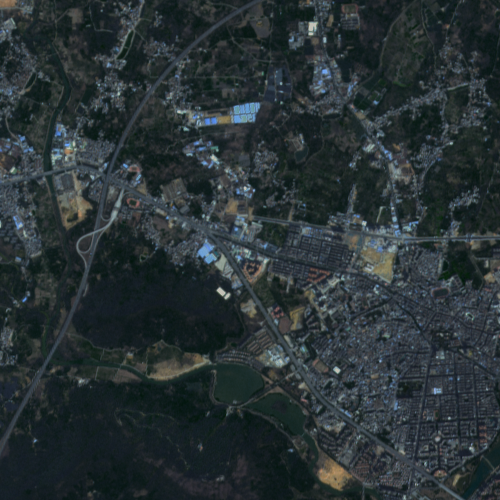
\includegraphics[height=2.5cm]{pic/pic01_mvgd.png}}
        \label{fig:0101}
        \caption{color transfer result}
    \end{figure}  
\end{frame}




